% DISTRIBUTION STATEMENT A. Approved for public release. 
% Distribution is unlimited.
%  
% This material is based upon work supported by the Defense Advanced Research 
% Projects Agency under Air Force Contract No. FA8702-15-D-0001. Any opinions, 
% findings, conclusions or recommendations expressed in this material are those 
% of the author(s) and do not necessarily reflect the views of the Defense 
% Advanced Research Projects Agency.
% 
% © 2019 Massachusetts Institute of Technology.
% 
% Subject to FAR52.227-11 Patent Rights - Ownership by the contractor (May 2014)
% 
% The software/firmware is provided to you on an As-Is basis
% 
% Delivered to the U.S. Government with Unlimited Rights, as defined in DFARS 
% Part 252.227-7013 or 7014 (Feb 2014). Notwithstanding any copyright notice, 
% U.S. Government rights in this work are defined by DFARS 252.227-7013 or 
% DFARS 252.227-7014 as detailed above. Use of this work other than as 
% specifically authorized by the U.S. Government may violate any copyrights 
% that exist in this work.

\chapter{Introduction}

The Lincoln Laboratory Ad-hoc MIMO Adaptive Communication
(LLAMAComm) simulation tool is a software package written in MATLAB.
It is designed to provide a framework for simulating cognitive MIMO
communication links in the presence of interference.  Cognitive
radios pose a special challenge because they scavenge for unused
bands in a wide range of frequencies.  These frequency bands contain
different types of interference sources which also need to be
simulated.

Users of this software package write functions that define the
physical and link layers of a radio under development.  LLAMAComm
takes these functions and applies propagation models to simulate the
transmission of the radio signal waveform.  It also coordinates the
simulation so that multiple radios may be simulated simultaneously.

%LLAMAComm is an upgrade to the Cogcom simulation software.  New
%features include the ability to simulate true forward and reverse
%links, asynchronous transmission, more flexible simulation
%structure, improved memory management, and better parameter
%organization.  Please note that MATLAB code written for Cogcom is
%not compatible with LLAMAComm.

%This introduction provides an overview to LLAMAComm and lists the
%major changes since Cogcom.  The following chapter illustrates the
%use of LLAMAComm by walking through the example simulation provided
%with the code.  This example will also illustrate how to port
%existing Cogcom code to LLAMAComm.  Detailed documentation on the
%inner workings of the simulator and the propagation models are
%provided in the final chapters.

%\section{What's New in LLAMAComm}

%\begin{figure}[h]
%\centering
%\mbox{
%    \subfigure[Cogcom]{\includegraphics[width=3in]{"figs/Cogcom
%    Scenario"}} \quad
%    \subfigure[LLAMAComm]{\includegraphics[width=3in]{"figs/LLAMAComm
%    Scenario"}}
%    }
%\caption{Comparison of Cogcom and LLAMAComm scenarios}
%\label{fig:compFig}
%\end{figure}

%LLAMAComm adds a number of features not found in Cogcom. Figure
%\ref{fig:compFig} illustrates the difference in complexity between a
%Cogcom scenario and a LLAMAComm scenario.  The LLAMAComm scenario
%contains multiple transmitters using possibly different frequencies
%with various transmission schemes.  In contrast, Cogcom was designed
%to simulate a single transmitter/receiver pair and a single in-band
%interferer using a rigidly defined transmission scheme. Table
%\ref{tbl:compTbl} lists the major differences between Cogcom and
%LLAMAComm.

%\begin{table}[h]
%\caption{Comparison of features between Cogcom and LLAMAComm}
%\label{tbl:compTbl}
%\begin{center}
%\begin{tabular}{|p{2.75in}|p{2.75in}|}
%  \hline \textbf{Cogcom v4.0} & \textbf{LLAMAComm} \\
%  \hline\hline
%    Simulates single MIMO link in the presence of interferers &
%    Simulates multiple simultaneous MIMO links in the presence of
%    interferers\\
%  \hline Simulates link in forward direction only &
%    Simulates forward and reverse links in the presence of interferers
%    that completely or partially overlap receive band \\
%  \hline Transmitter and receiver always synchronized &
%    Possible to transmit asynchronously.  Propagation delay
%    simulated \\
%  \hline Simulation structure fixed.  No control of link layer
%    allowed &
%    Flexible software structure allows simulation of link layer and ad-hoc
%    networks \\
%  \hline &
%    Improvements to memory management to allow longer simulations \\
%  \hline &
%    Simplified simulation parameter configuration \\
%  \hline
%\end{tabular}
%\end{center}
%\end{table}

\section{Software Overview}

Many features are realized by making the structure of the
simulator \emph{generalized}.  LLAMAComm simulations are built
around the notion of a node.  Nodes represent radios.  The nodes are
meant to be self-contained; nodes do not share information with
other nodes and can only communicate through the wireless channel.

To run a simulation, nodes are thrown into an environment by
defining their position in a configuration file.  The simulator then
interacts with the nodes to automatically coordinate the execution
of the simulation.  The propagation model and coordination between
various transmitting and receiving nodes are taken care of by
LLAMAComm.

Nodes in LLAMAComm are implemented as MATLAB objects.  The node
objects contain a list of parameters, module objects (which describe
the radio interface), and a controller function. Figure
\ref{fig:softwareOverview} illustrates how a scenario consisting of
two FM transceivers and an interfering FM transmitter would be
implemented in the simulator. User A, User B, and the FM interferer
(labeled \verb+Interference+) are all node objects.

The user-defined node objects contain two module objects each: FM Tx
and FM Rx.  Module objects contain functions that implement the
physical layer of the radio.  The transceivers here might use BPSK
with a 1 MHz bandwidth, so functions in FM Tx would contain a BPSK
modulator and some simple filters.  These modules can be reused
between different nodes.  In this example, User B uses the same FM
modulator and demodulator as User A.

\begin{figure}[h]
\centering
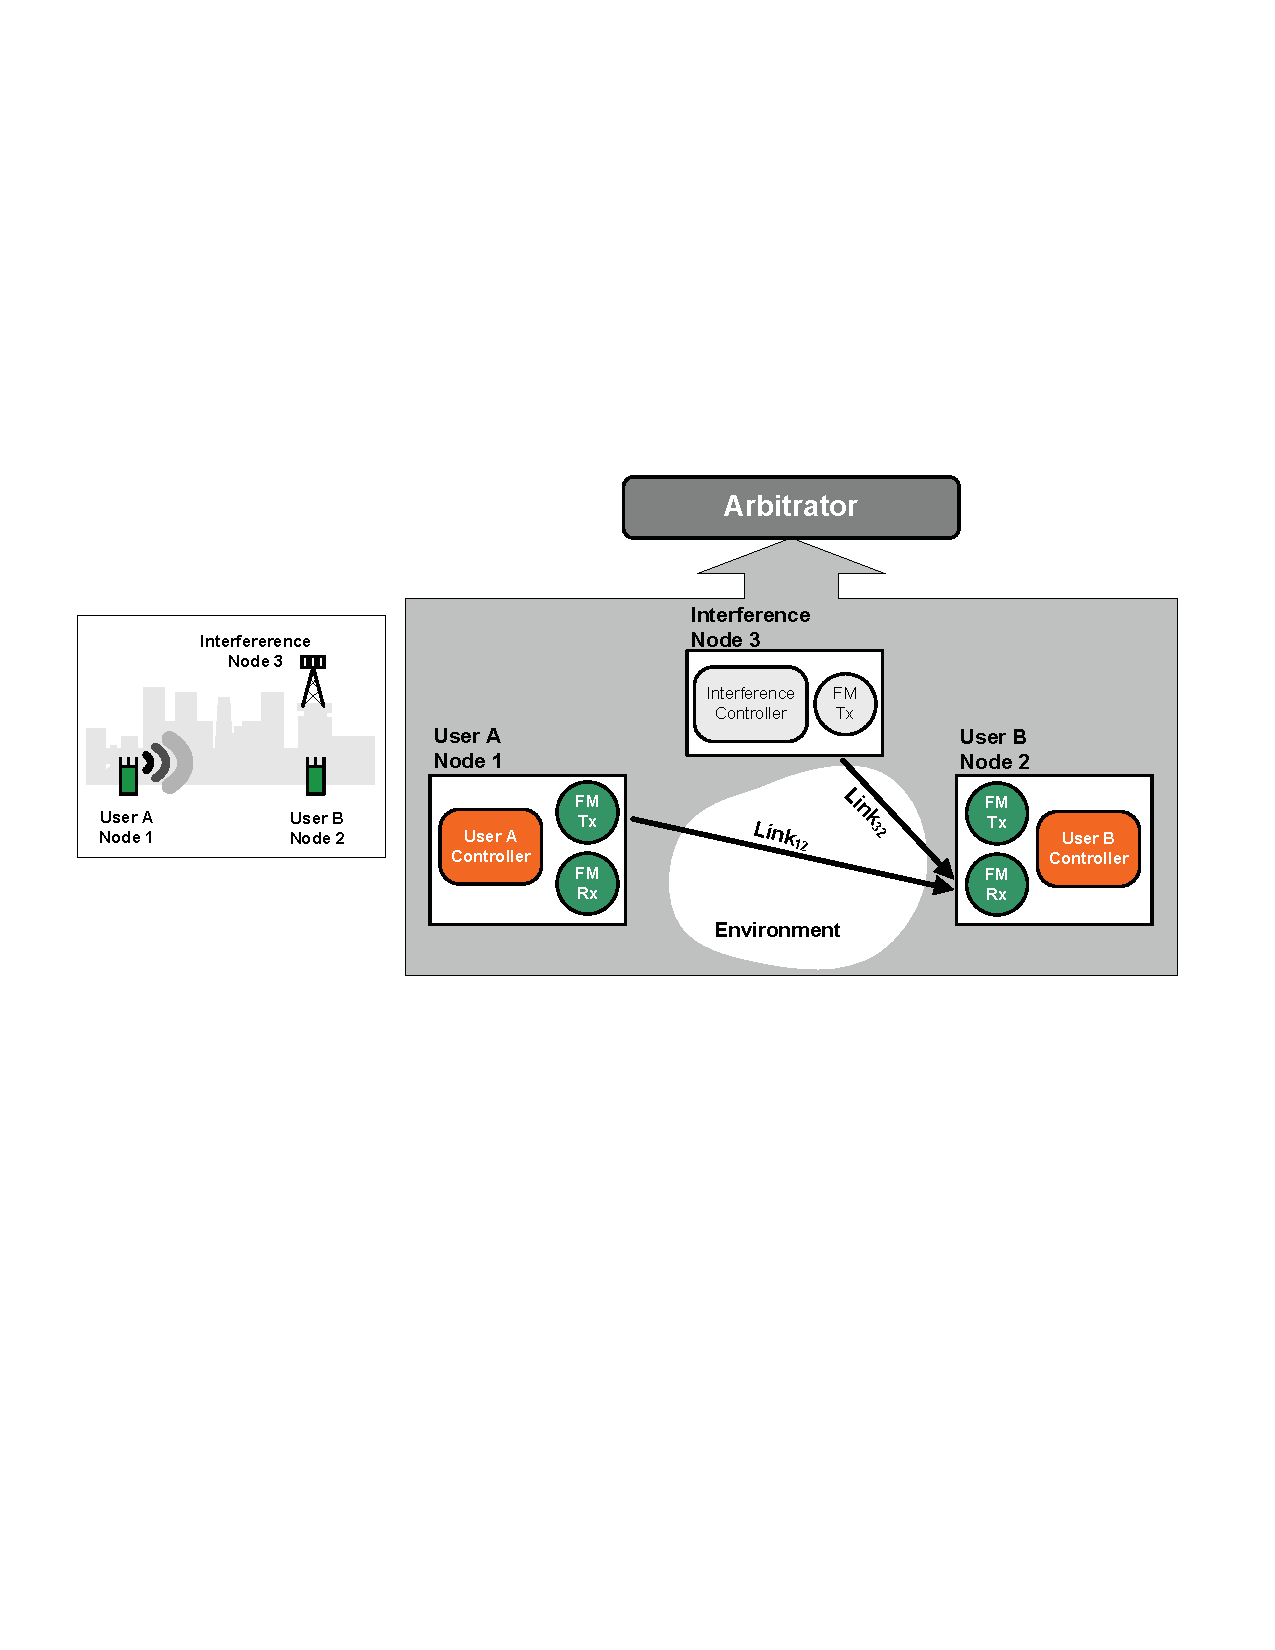
\includegraphics[width=6in]{figs/Software_Overview}
\caption{Example of how a scenario relates to software structure}
\label{fig:softwareOverview}
\end{figure}

The controller functions are state machines written in a specific
way so that they can coordinate with the LLAMAComm arbitrator.  The
coordination is handled through a request/acknowledge system.  Nodes
that wish to transmit or receive a segment of analog signal must
send a request to the arbitrator containing the segment start time
and segment duration.  The arbitrator coordinates execution order so
that any possible interference is included in a segment of received
signal.  In practice, this coordination is transparent to the user.

The remaining portions of the simulation---including the environment
and link objects---are created by the simulator and operate in the
background.  Basically, the user is responsible for programming the
portions of Figure \ref{fig:softwareOverview} that are in color.
Since LLAMAComm includes some pre-made interference sources, this
example would require the user to write only four MATLAB functions:
the FM transmit module, FM receive module, User A controller, and
User B controller.

This is a simple example, intended as a quick overview.  A more
complicated scenario would contain more nodes, and each node may
contain more than two modules.  There are also other features of the
simulator not yet mentioned, such as the special ``genie'' link.
These details, and more, are covered in the following chapters.

% DISTRIBUTION STATEMENT A. Approved for public release. 
% Distribution is unlimited.
%  
% This material is based upon work supported by the Defense Advanced Research 
% Projects Agency under Air Force Contract No. FA8702-15-D-0001. Any opinions, 
% findings, conclusions or recommendations expressed in this material are those 
% of the author(s) and do not necessarily reflect the views of the Defense 
% Advanced Research Projects Agency.
% 
% © 2019 Massachusetts Institute of Technology.
% 
% Subject to FAR52.227-11 Patent Rights - Ownership by the contractor (May 2014)
% 
% The software/firmware is provided to you on an As-Is basis
% 
% Delivered to the U.S. Government with Unlimited Rights, as defined in DFARS 
% Part 252.227-7013 or 7014 (Feb 2014). Notwithstanding any copyright notice, 
% U.S. Government rights in this work are defined by DFARS 252.227-7013 or 
% DFARS 252.227-7014 as detailed above. Use of this work other than as 
% specifically authorized by the U.S. Government may violate any copyrights 
% that exist in this work.
